\section{Results}
\subsection{Verification Problem I}
A comparison between the  radionuclide production collected in cell,
and meshes of sizes 1x1x1, 2x2x2, and 4x4x4 laid in the same geometric cell
was done. The mesh results were added across all mesh volumes for a direct
comparison to the cell results. These are shown in Figure \ref{fig:1prod_cell_2x_4x}
\begin{figure}[h!]
 \begin{centering}
 \centering
 \begin{subfigure}[b]{.8\textwidth}
 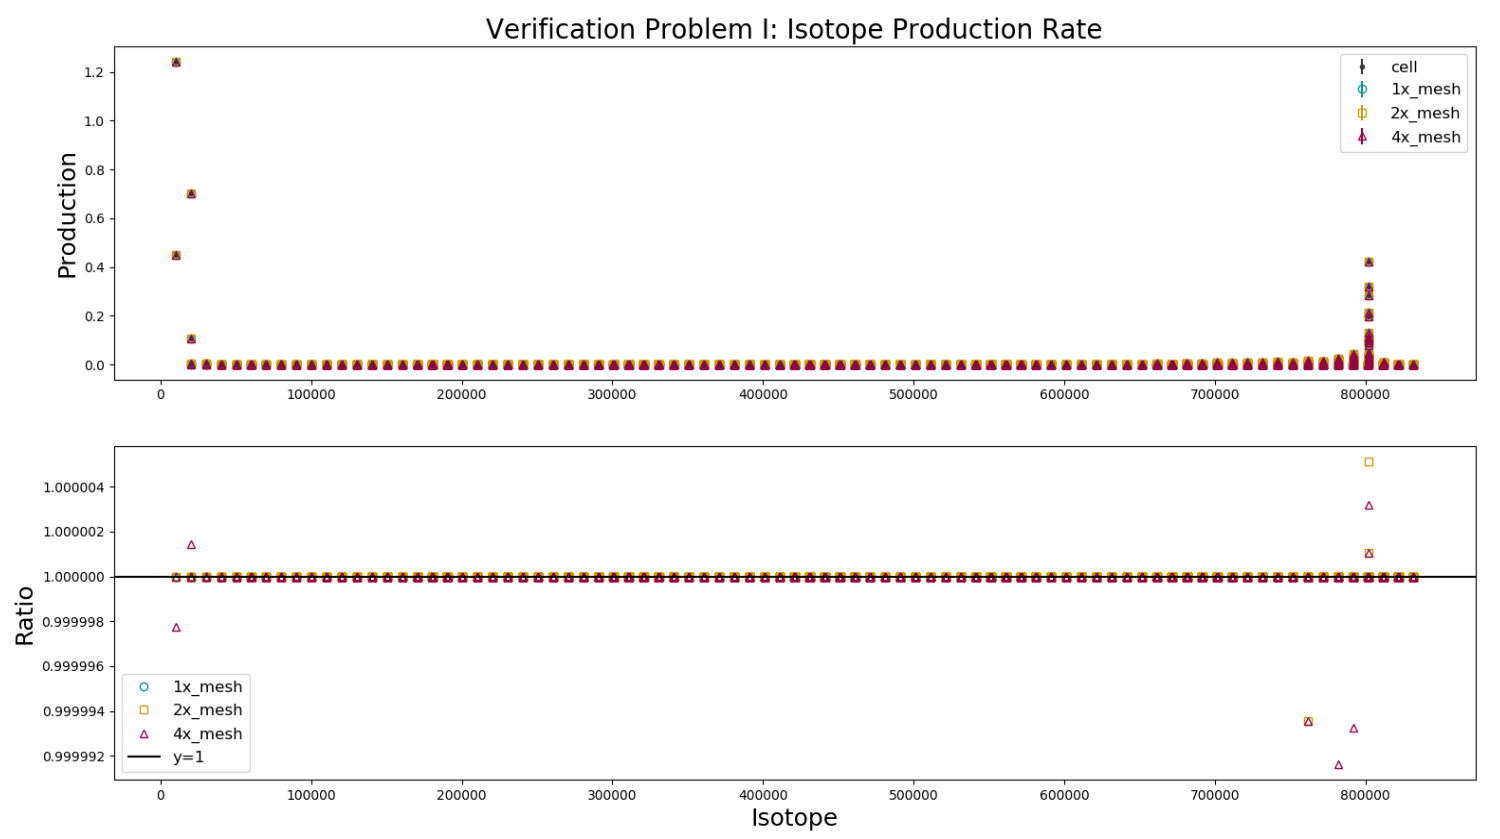
\includegraphics[width=0.99\linewidth,height=8cm]{../figs/toy_p1/prod_VPI_1x_2x_4x.png}
 \caption{Radionuclide production rates}
 \label{fig:1prod_cell_2x_4x}
 \end{subfigure}
 \hspace{0.05cm}
 %
 \begin{subfigure}[b]{.8\textwidth}
 \centering
 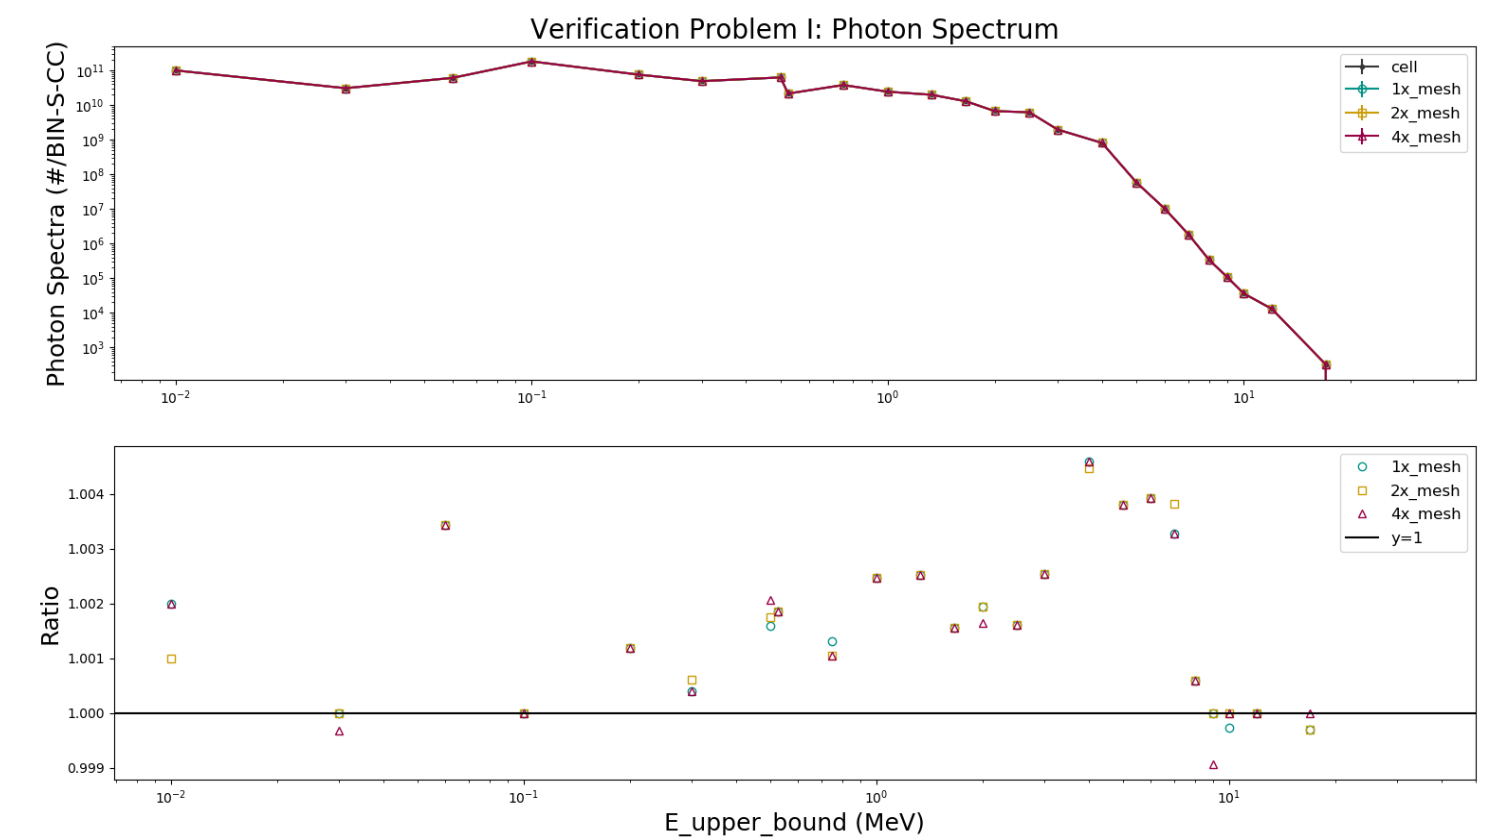
\includegraphics[width=.99\linewidth,height=8cm]{../figs/toy_p1/spec_VPI_1x_2x_4x.png}
 \caption{Photon emission rate at 1 minute decay }
 \label{2prod_cell_2x}
 \end{subfigure}
 \caption{Verification Problem I: Comparison between results for geomtric cell, and different size meshes}
 \label{prod_cell_2x}
 \end{centering}
\end{figure}
%%
A comparison of the radionuclide production between a cell rnucs,
meshed rnucs, and geometry split rnucs  for Verification Problem
I and Verification problem II are shown in Figures
\ref{1prod_cell_2x} and \ref{2prod_cell_2x} respectively.\\
A comparison between the radionuclides in a cell, and the sum or average of the 
\begin{figure}[h!]
 \begin{centering}
 \centering
 \begin{subfigure}[b]{.8\textwidth}
 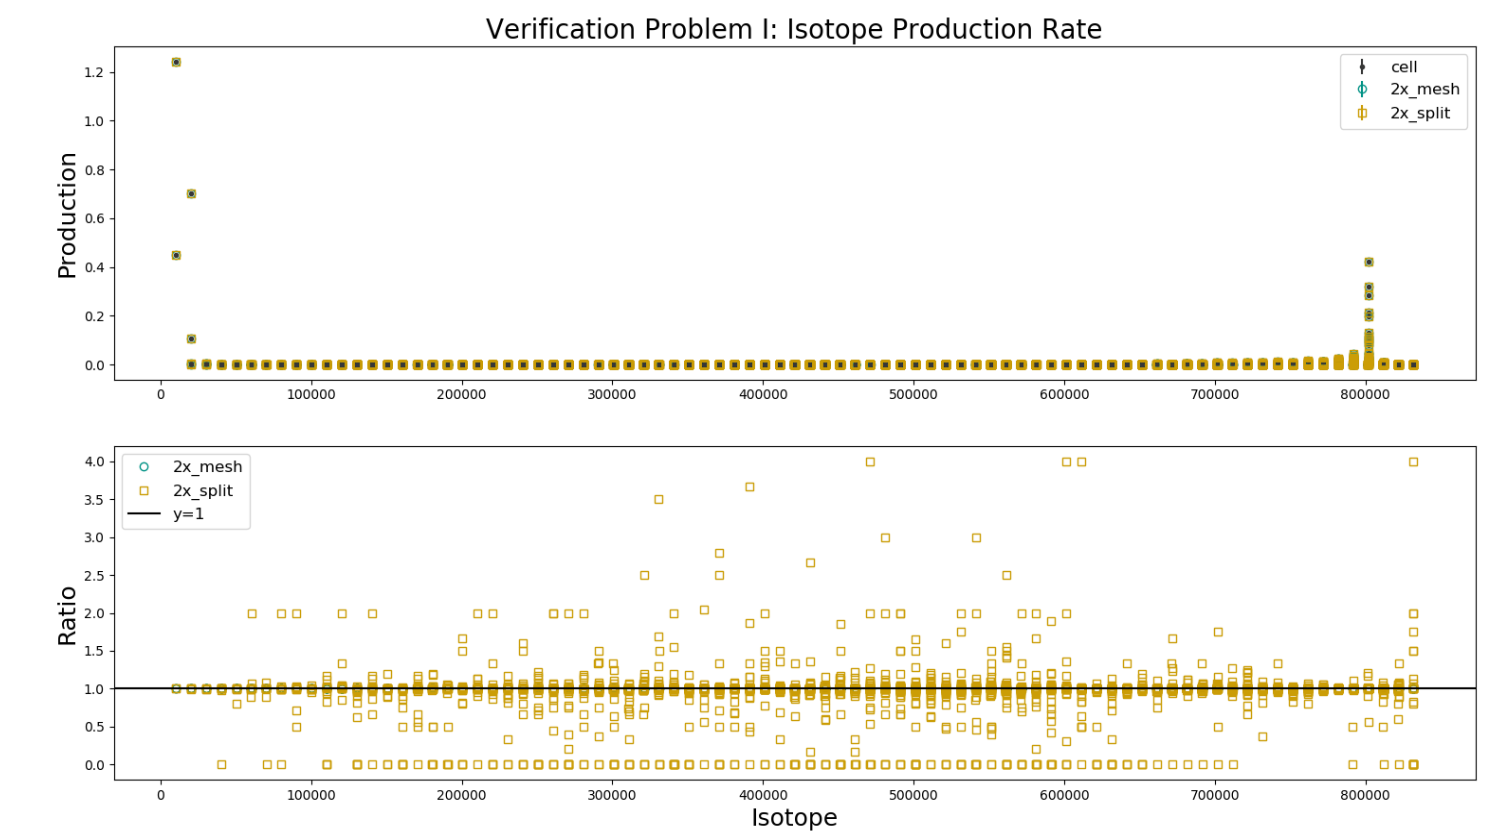
\includegraphics[width=0.99\linewidth,height=8cm]{../figs/toy_p1/prod_VPI_2x.png}
 \caption{Verification problem I }
 \label{1prod_cell_2x}
 \end{subfigure}
 \hspace{0.05cm}
 %
 \begin{subfigure}[b]{.8\textwidth}
 \centering
 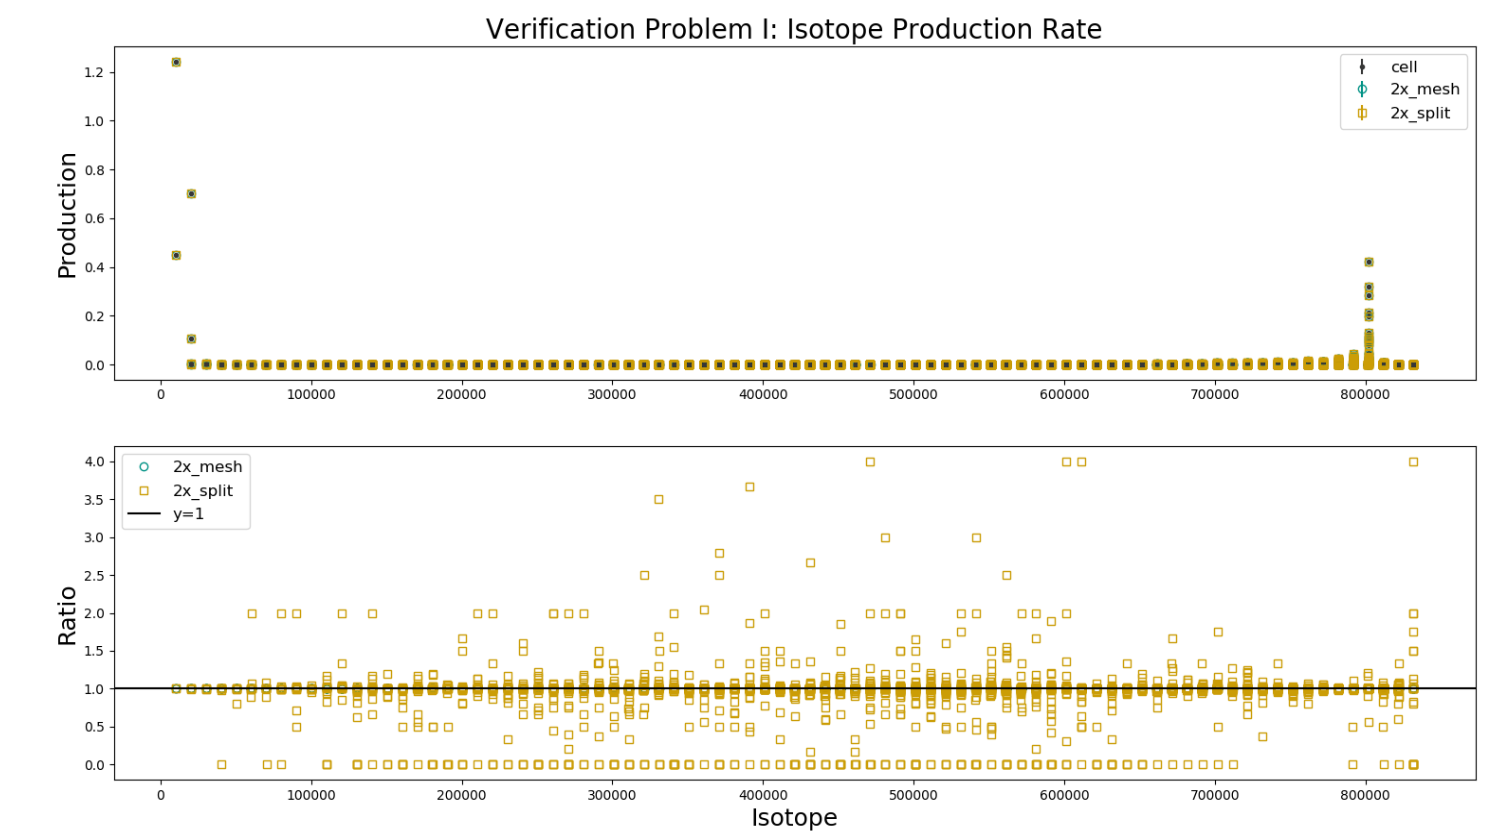
\includegraphics[width=.99\linewidth,height=8cm]{../figs/toy_p1/prod_VPI_2x.png}
 \caption{Verification problem II}
 \label{2prod_cell_2x}
 \end{subfigure}
 \caption{Radionuclide production for cell, meshed and split geometries}
 \label{prod_cell_2x}
 \end{centering}
\end{figure}
%%
Figures \ref{1spect_cell_2x} and \ref{2spect_cell_2x} show a similar
comparison for the photon spectrum.\\
\begin{figure}[h!]
 \begin{centering}
 \centering
 \begin{subfigure}[b]{.45\textwidth}
 \includegraphics[width=0.95\linewidth,height=5cm]{../figs/toy_p1/1spectrum_cell_2x_t32.png}
 \caption{Verification problem I }
 \label{1spect_cell_2x}
 \end{subfigure}
 \hspace{0.05cm}
 %
 \begin{subfigure}[b]{.45\textwidth}
 \centering
 \includegraphics[width=.95\linewidth,height=5cm]{../figs/toy_p2/2spectrum_cell_2x_t32.png}
 \caption{Verification problem II}
 \label{2spect_cell_2x}
 \end{subfigure}
 \caption{Photon Spectrum at 1hr after shutdown }
 \label{spect_cell_2x}
 \end{centering}
\end{figure}
Figures \ref{prod_cell_2x} and \ref{spect_cell_2x} suggest that the splitting the geometries 
differs the most from the original rnucs workflow. In this particular case, splitting the geometry 
into 8 equal parts for Verification problem II required material mixing.
This is likely to show in the large discrepancy between the cell case and the split case.
Another important comparison is that of the cell rnucs with the progression of the mesh rnucs. 
Figure \ref{voxels} shows the order of the voxels used in Figure \ref{spect_cell_2x_byV}. 


\begin{figure}[h]
\begin{centering}
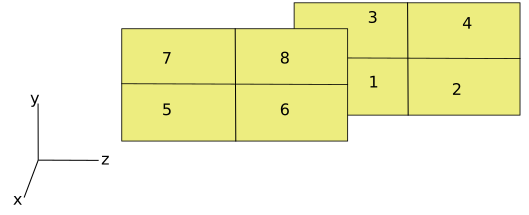
\includegraphics[width=0.60\linewidth]{../figs/voxels.png}
\caption{Voxel configuration}
\label{voxels}
\end{centering}
\end{figure}

\begin{figure}[h]
 \begin{centering}
 \centering
 \begin{subfigure}[b]{.45\textwidth}
 \includegraphics[width=0.95\linewidth,height=5cm]{../figs/toy_p1/1spectrum_cell_2x_byV_t32.png}
 \caption{Verification problem I }
 \label{1spect_cell_2x_byV}
 \end{subfigure}
 \hspace{0.05cm}
 %
 \begin{subfigure}[b]{.45\textwidth}
 \centering
 \includegraphics[width=.95\linewidth,height=5cm]{../figs/toy_p2/2spectrum_cell_2x_byV_t32.png}
 \caption{Verification problem II}
 \label{2spect_cell_2x_byV}
 \end{subfigure}
 \caption{Photon Spectrum at 1hr after shutdown for each voxel in a 2x2x2 mesh}
 \label{spect_cell_2x_byV}
 \end{centering}
\end{figure}
In Figure \ref{spect_cell_2x_byV} there are three distinct set of the lines, the 
first one is the one for the cell, the second set belong to voxels 1, 3, 5, and 7, and the 
last group belongs to voxels 2, 4, 6, and 8. Voxels 1, 3, 5, and 7 have greater photon emission 
than the voxels 2, 4, 6, and 8. This is expected as the source is to the left of the geometry. 
Having a mesh gives more spatial definition which is useful for large geometric cells. 
\newpage
